\documentclass{article}
\usepackage{biblatex}
\usepackage{url}
\usepackage{graphicx}


\title{Angry Birds}
\author{Kamalkorak Adhikari}

\bibliography{references}
\addbibresource{references.bib}


\begin{document}
\maketitle
\section{Introduction}
It is a modified version of the game Angry Birds.
Instead of being single player, it is a multiplayer turn-based game.
The goal of the game is to destroy all the blocks.Whoever finishes the game first or has highest score before time out wins.
\section{Features}
The game has the following features:
\begin{itemize}
    \item Two player game : The game is designed for two players. Each player takes turns to play the game.
    \item Bird selection : The game allows the players to select their birds (4 types).Each bird deals different damage depending on the type of block.
    \item Level selection : The game allows the players to select the level of the game. The players can choose from a variety of levels.
    \item Wind impulse mode : The game allows the players to select the wind impulse mode. A random wind direction is set in each round.\newline \emph{Not reflected in the predicted projectile path.}
    \item Projectile path : The game shows the projectile path of the bird. The players can see the trajectory of the bird before launching it.
    \item Game sounds : The game has various background and event sounds. The sounds are used to enhance the gaming experience.
    \item Destruction stages : The game has destructible blocks. The blocks have health points. 5 stages of destruction are implemented.
    \item Falling blocks : The game has falling blocks. The blocks fall when the lower support is destroyed.
    \item Score system : The game has a score system. Destruction of blocks gives points to the player and the highest score is stored.
    \item CountDown timer : The game has a countdown timer.
\end{itemize}
\pagebreak
    \section{Game Mechanics I (On the Surface)}
\subsection{modules}
The project utilizes the following modules:
\begin{itemize}
    \item pygame : This is the main module used for creating the game.
    \item random : This module is used to generate random numbers for the game.
    \item math : This module is used for mathematical calculations.
    \item time : This module is used to control the time in the game.
    \item sys : This module is used to control the system.
\end{itemize}

\subsection{Game Loop}
The game loop is the main part of the game. It is responsible for updating the game state and rendering the game on the screen. The game loop runs continuously until the game is over.


\subsection{Game States}
The game state is a dictionary that contains the current state of the game. It includes the following
information:
\begin{itemize}
    \item state [0] : Game starts and the players are prompted to enter their names. Event for loop takes care of the names input.
    \item state [-1 \& -2] : Innitial bird choice window -1 for player 1 and -2 for player 2.
    \item state [-3] : Level choice window. The player is prompted to choose a level.
    \item state [-4] : Chaice for wind impulse mode
    \item state [-5] : A short interval temporary state for clearing the screen before the game starts. Once finished gamestate is set to 1.
    \item state [1] : The game is in progress. Player 1 is allowed to make a move. Once the turn is over, the game state is set to 2.
    \item state [2] : The game is in progress. Player 2 is allowed to make a move. Once the turn is over, the game state is set back to 1.
    \item state [3] : The game is over. The player who finished the game first wins (Victory screen)
\end{itemize}
\pagebreak
\subsection{Visual Elements}
The graphic elements (sprites) are extracted from \cite{Sprites} and \cite{wiki}
The game uses the following visual elements:
\begin{itemize}
    \item Selection window : The selection window is used to select the level of the game.
    \item Bird selection window : The bird selection window is used to select the bird of the game. It is used to display the birds of the game.
    \item Background : The background is the main visual element of the game. It is used to create the game environment.
    \item Bird : The bird is the main character of the game. It is used to destroy the blocks.
    \item Block : The block is the main object of the game. It is destructed by the bird.
    \item Block health : The block health is used to show the health of the block.
    \item Slingshot : The slingshot is used to launch the bird. It supports extension and contraction of the rubber band.
    \item Projectile path : The projectile path is used to show the path of the bird. It is used to show the trajectory of the bird.
    \item Victory window : The Victory window is used to display the winner of the game.
\end{itemize}

\subsection{Game sound}
The game uses various background and event sounds.
This is done using the pygame.mixer module. This sounds are extracted from \cite{Sounds}

\subsection{Game Objects}
The game objects are the main components of the game. They include the following:
\begin{itemize}
    \item Bird : The bird is the main character of the game. It is used to destroy the blocks.It is handled by Ball class.
    \item Block : The block is the main object of the game. It is destructed by the bird.It is handled by StaticObstacle class.
\end{itemize}
\pagebreak
\section{Game Mechanics II (Under the Hood)}
\subsection{Collision Logic}
The collision logic is used to detect the collision between the bird and the block. It is used to check if the bird has hit the block. The collision logic is implemented using the following methods:
\begin{itemize}
    \item method collision : This method is used to check if the bird has hit the block. It updates the direction and speed of the bird and the health of the block.
    \item method window\_collision : This method is used to check if the bird has hit the window. It updates the direction of the bird.
\end{itemize}
The methods are called in the respective instances of ball class in update method. The update method is called in the game loop.

\subsection{Collision direction}
\begin{flushleft}
    It is the fundamental part of collision logic and is used to determine the direction.As per \cite{Collisions}, it is determined using the following principles:\linebreak \linebreak
For the ball objects two rect positions are maintained.\newline The primary rect (current position) and the old\_rect
The pygame collision only detects an overlap between the two objects. It does not provide the direction of the collision.
\linebreak
Whenever there is a collision, the primary rect overlaps but the old rect does not as it's update is called after handling the collision.
\linebreak
Now taking example of left to right collision of ball that is the ball hitting the left side of the block.
\newline
We check
\begin{equation}
    Primary\_ball\_right\_margin > block\_left\_margin
\end{equation}
\begin{equation}
    Old\_rect\_ball\_right\_margin < block\_left\_margin
\end{equation}
This ensures that the ball was on the left side of the block before collision.
\newline
The same principle is applied to all the other directions.
\end{flushleft}

\subsection{Collision grouping}
It is essential to ensure that the birds of player 1 hit only the blocks of player 2 and vice versa.
\newline
To achieve this, the birds and blocks are grouped into two groups. The birds of player 1 and the blocks of player 2 are grouped into group 1. The reverse is done for player 2.
(The sprite grouping process is handled by pygame)
\pagebreak
\subsection{Projectile path}
The projectile path is used to show the trajectory of the bird. The projectile path is implemented using the following equations:
\begin{equation}
    range(x) = V_x * T
\end{equation}
\begin{equation}
    height(y) = \frac{V_y^2}{2g}
\end{equation}
\begin{equation}
    T = \frac{2 * V_y}{g}
\end{equation}
Since, the projectile path is a parabola, with range and height as the two axes, we can use the pygame.draw.arc method to draw the projectile path.

\subsection{Some other methods and attributes}
\begin{itemize}
    \item spriteSetup() : This method is used to set up the sprites of the game. It is used to create the bird and block objects by checking given parameters.
    \item step() : This method is used to load random birds for the players alternatively once initial birds are terminated.
    \item attribute self.type : For both birds and blocks, this attribute is used to determine the type of the object and extract the required parameters from const.py
    \item const.py : This file stores the addresses of the sprites used in various objects and also the level designs.
\end{itemize}

\section{Directory Structure}
AngryBirds \newline
--- main.py         //main executable file\newline
--- const.py        //stores important addresses\newline
--- resources\newline
-------- images\newline
-------- sound\newline
-------- img\newline
-------- ComicSansMS3.ttf\newline
--- documentation\newline
-------- Report.tex\newline
-------- Report.pdf\newline
-------- references.bib\newline
\pagebreak
\section{Running Instructions}
Just run python3 main.py or python main.py in the terminal depending on os.The player is prompted to enter the names and select the birds, levels and game mode. The game starts after that.\newline
Click on the bird, drag it away from the slingshot and release the mouse to launch it. The player can see the projectile path before launching the bird.

\section{Project Journey}
It has been a great experience working on this project. I have learned a lot about game development and the pygame module especially about collision detection and how to implement it in a game. I have also learned about the importance of sound and visual elements in a game and how to impliment them to enhance the gaming experience.
\newline
Although it was fun, the first 2 days were very difficult. I was scrolling though documentations and youtube tutorials to understand the pygame module. After day and night of scrattching my head, I was able to understand the basics of the module.
\newline
Day 3: Things started to get clear and easier to understand.
\newline
Day 4: Once the core collision system started working properly, rest of the work became much smoother.
\newline
Day 5 and onwards: Refining smoothening and adding optional features.

\begin{figure}[h]
    \centering
    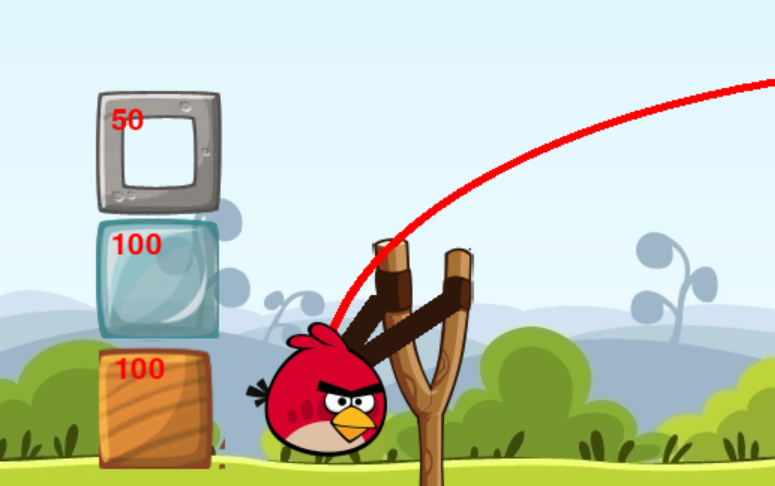
\includegraphics[width=0.8\textwidth]{Screenshot.png}
    \caption{Screenshot}
    \label{fig:game_window}
\end{figure}

\pagebreak

\printbibliography[heading=bibintoc]

\end{document}